\documentclass{standalone}
\usepackage{tikz}
\usetikzlibrary{shapes, arrows}

% diagram elements
\tikzstyle{base} = [draw, minimum height=2em, text centered, text width=6em]
\tikzstyle{terminator} = [base, rectangle, rounded corners]
\tikzstyle{process} = [base, rectangle, fill=yellow!20]
\tikzstyle{decision} = [base, diamond, fill=blue!20]
\tikzstyle{data} = [base, trapezium, trapezium left angle=60, trapezium right angle=120]
\tikzstyle{data input}=[data, fill=red!20]
\tikzstyle{data output}=[data, fill=green!20]
\tikzstyle{connector} = [draw, -latex']
\tikzstyle{connector text} = [midway, above, xshift=4mm, text=black]

\begin{document}
	
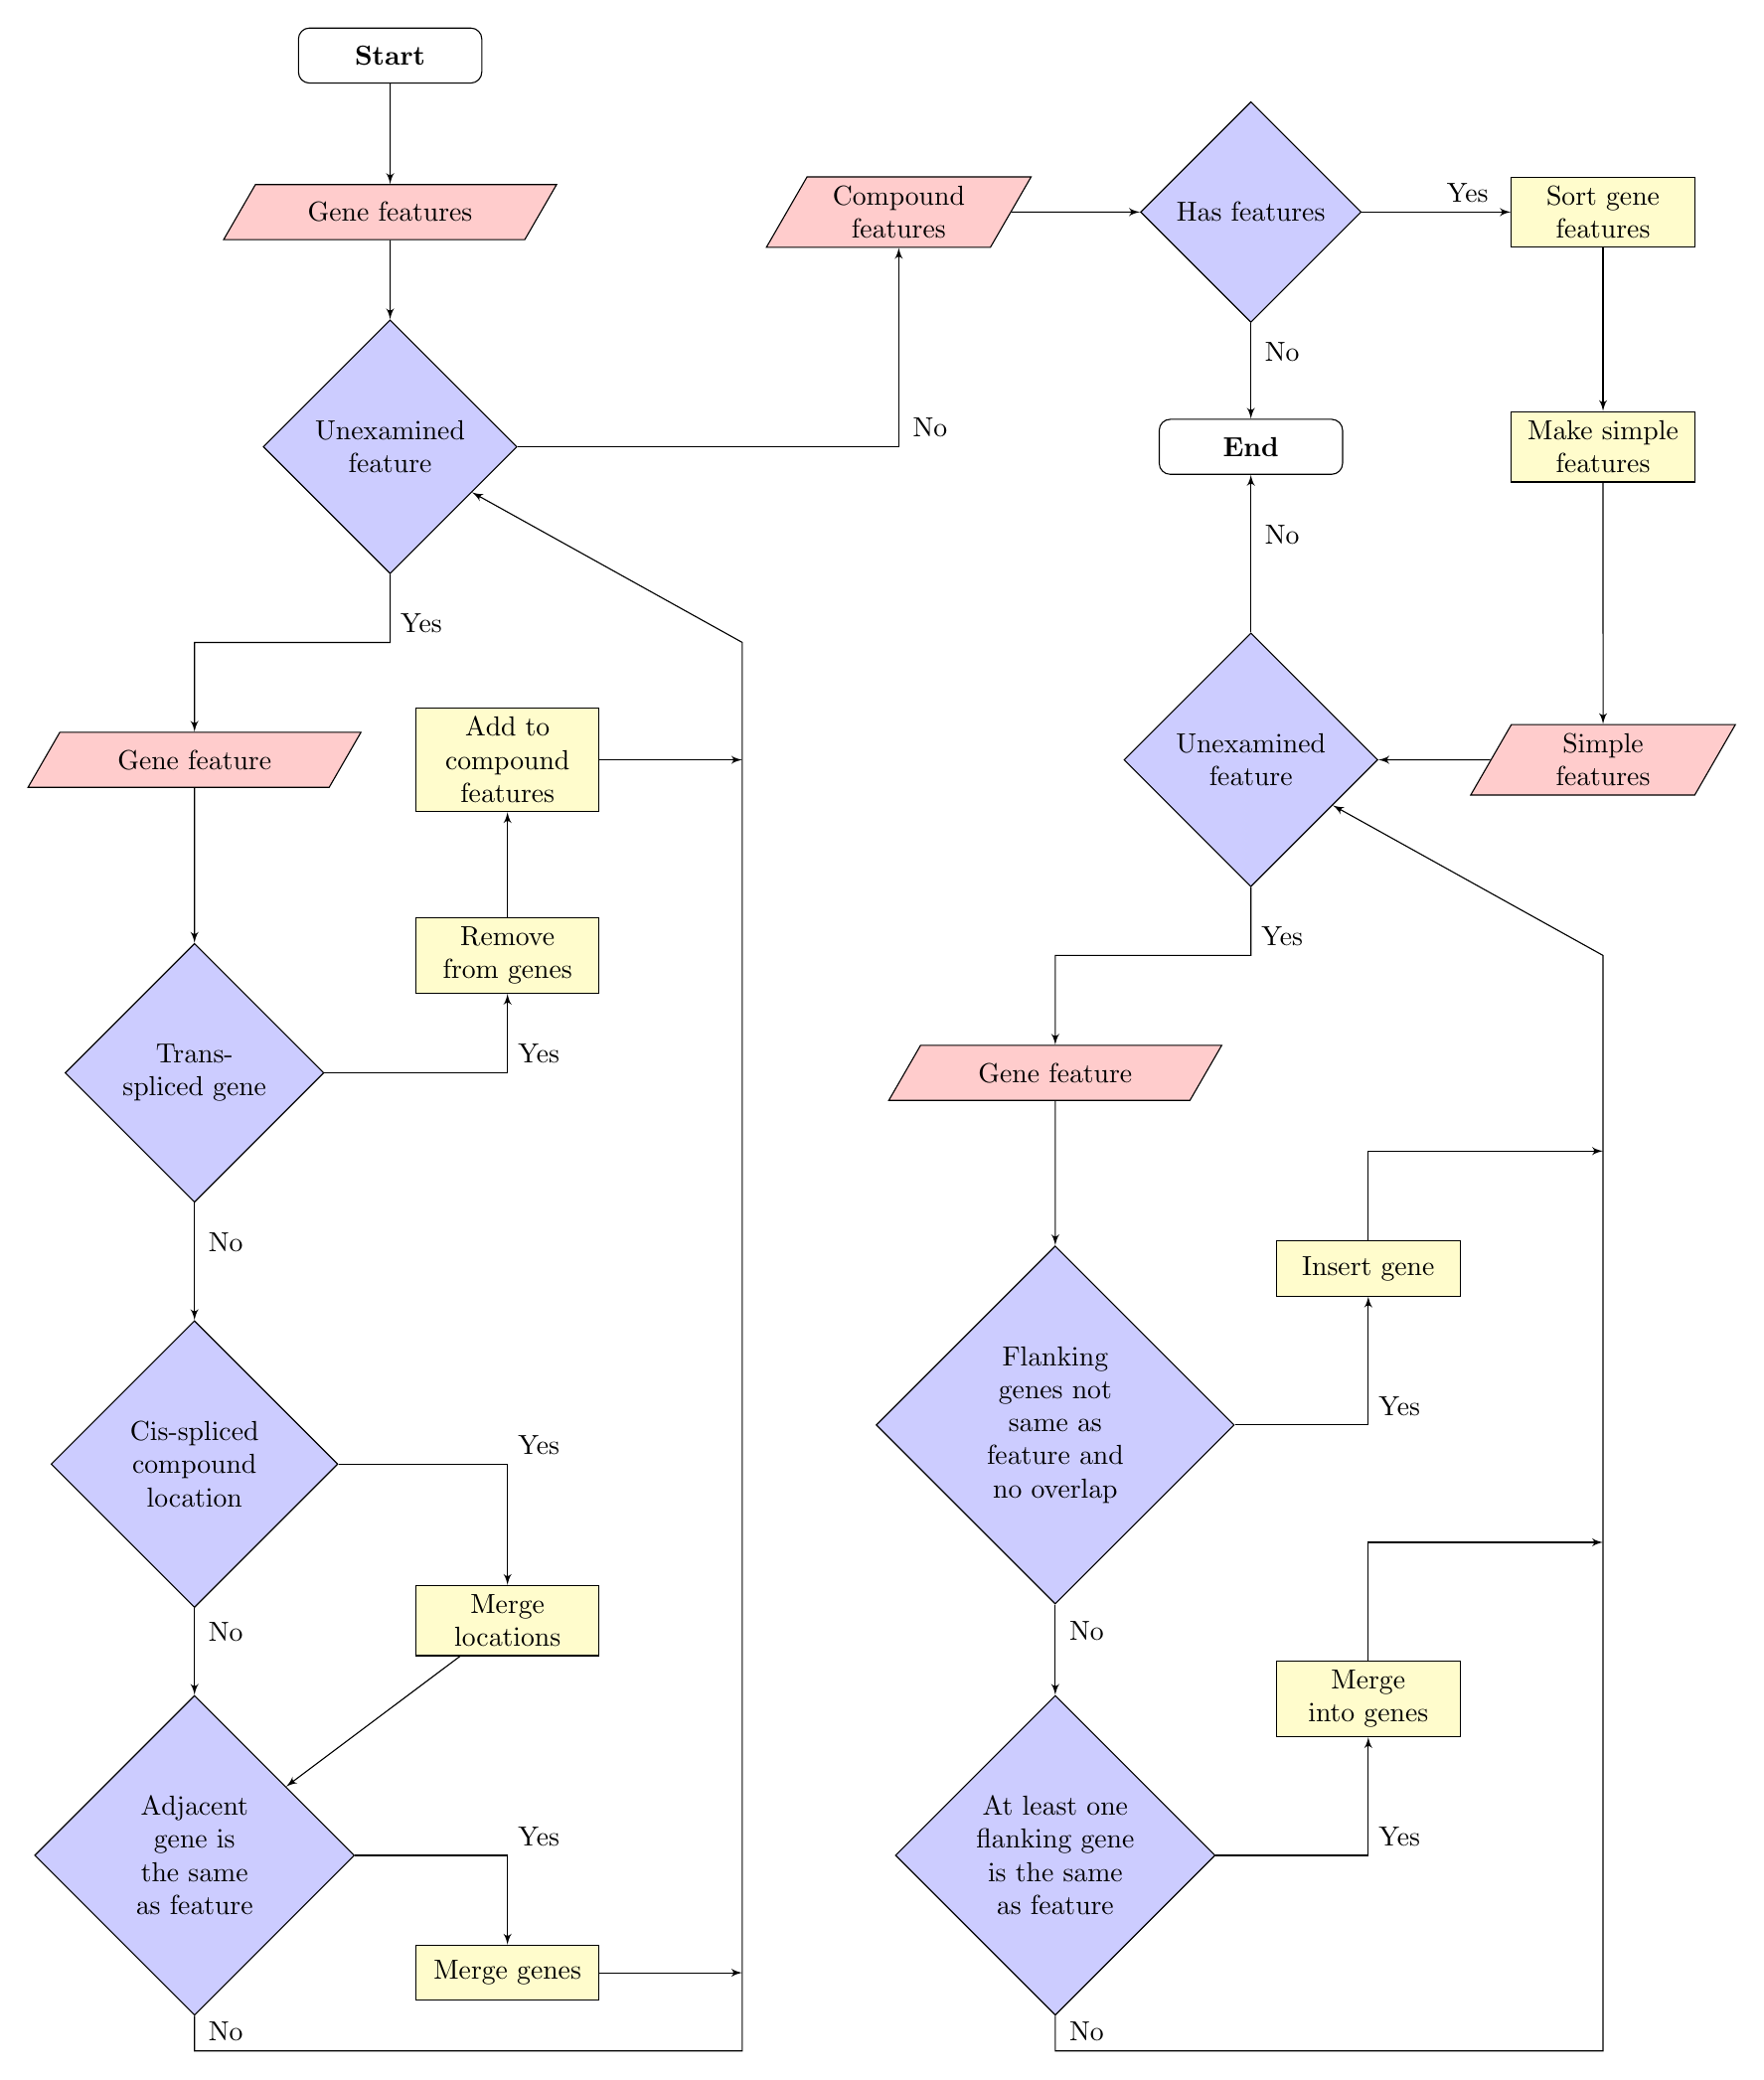
\begin{tikzpicture}
	
	\node [terminator] at (-1.5, 0) (start) {\textbf{Start}};
	\node [terminator] at (9.5, -5) (end) {\textbf{End}};
	
	% exon split merger
	\node [data input] at (-1.5,-2) (genes) {Gene features};
	\node [data input] at (-4, -9) (gene) {Gene feature};
	
	\node [decision] at (-1.5,-5) (feature) {Unexamined feature};
	\node [decision] at (-4,-13) (trans) {Trans-spliced gene};
	\node [decision] at (-4,-18) (compound) {Cis-spliced compound location};
	\node [decision] at (-4,-23) (adjacent) {Adjacent gene is the same as feature};
	
	\node [process] at (0, -11.5) (remove) {Remove from genes};
	\node [process] at (0, -9) (add compound) {Add to compound features};
	\node [process] at (0, -20) (merge cis) {Merge locations};
	\node [process] at (0, -24.5) (merge adj) {Merge genes};
	
	\path [connector] (start) -- (genes);
	\path [connector] (genes) -- (feature);
	\path [connector] (gene) -- (trans);
	\path [connector] (remove) -- (add compound);
	\path [connector] (add compound) -- (3, -9);
	\path [connector] (merge cis) -- (adjacent);
	\path [connector] (merge adj) -- (3,-24.5);
	
	\path [connector] (feature) |- node[connector text] {Yes} (-4, -7.5) -- (gene);
	\path [connector] (trans) -| node[connector text] {Yes} (remove);
	\path [connector] (compound) -| node[connector text] {Yes} (merge cis);
	\path [connector] (adjacent) -| node[connector text] {Yes} (merge adj);
	
	\path [connector] (trans) -- node[connector text] {No} (compound);
	\path [connector] (compound) -- node[connector text] {No} (adjacent);
	\path [connector] (adjacent) |- node[connector text] {No} (3, -25.5) -- (3, -7.5) -- (feature);
	
	% exon split insertor
	\node [data input] at (5,-2) (compound feats) {Compound features};
	\node [data input] at (14, -9) (simples) {Simple features};
	\node [data input] at (7, -13) (simple) {Gene feature};
	
	\node [decision] at (9.5, -2) (has compound) {Has features}; 
	\node [decision] at (9.5, -9) (has simple) {Unexamined feature};
	\node [decision] at (7, -17.5) (can insert) {Flanking genes not same as feature and no overlap};
	\node [decision] at (7, -23) (can merge) {At least one flanking gene is the same as feature};
	
	\node [process] at (14, -2) (sort) {Sort gene features};
	\node [process] at (14, -5) (make simples) {Make simple features};
	\node [process] at (11, -15.5) (insert) {Insert gene};
	\node [process] at (11, -21) (merge trans) {Merge into genes};
	
	\path [connector] (compound feats) -- (has compound);
	\path [connector] (sort) -- (make simples);
	\path [connector] (make simples) -- (simples);
	\path [connector] (simples) -- (has simple);
	\path [connector] (simple) -- (can insert);
	\path [connector] (insert) |- (14, -14);
	\path [connector] (merge trans) |- (14, -19);
	
	\path [connector] (has compound) -- node[connector text] {Yes} (sort);
	\path [connector] (has simple) |- node[connector text] {Yes} (7, -11.5) -- (simple);
	\path [connector] (can insert) -| node[connector text] {Yes} (insert);
	\path [connector] (can merge) -| node[connector text] {Yes} (merge trans);
	
	\path [connector] (feature) -| node[connector text] {No} (compound feats);
	\path [connector] (has simple) -- node[connector text] {No} (end);
	\path [connector] (has compound) -- node[connector text] {No} (end);
	\path [connector] (can insert) -- node[connector text] {No} (can merge);
	\path [connector] (can merge) |- node[connector text] {No} (14, -25.5) -- (14, -11.5) -- (has simple);
%	\path [connector] (can merge) -- (10.5,-23) node[connector text] {No} -- (14,-23) -| (14,-23) -- (14, -11.5) -- (11, -11.5) -- (has simple);
	
\end{tikzpicture}

\end{document}